\chapter{Background}
\label{ch:background}

The purpose of this section is to provide background information into the problem area, as well as introduce and explain concepts that will be used throughout the rest of the document.

\section{Current services}
\label{sec:current-services}
Understanding the current available applications and their limitations is important. It helps to narrow down the problem area, and identifies the requirements for the new system.

It is fair to say that there are a wide range of personal finance applications available, however, they are not all suitable for the same use case. For the purpose of this project, the focus is on those that help provide a user with an overview of their finances, as these are most applicable in improving a user's financial literacy. These existing tools can be divided into three main categories. Firstly, there are the applications that do not utilise open banking, and as such require manually importing the data. Secondly, there are the mobile banking applications that do use open banking, but instead often focus on single accounts, so not a big overview. Finally, there are applications which you often have to pay for, or a filled with advertisements and furthermore, lack analytics.

\subsection{Manual Importing Applications}
\label{sec:manual-importing-applications}
The first category of applications are those that do not use open banking. Often, these tools are older and lack updates which is why they haven't been improved to utilise the end points offered in open banking. The most prominent example of this GNU Cash \cite{GNUCash}. This is a free and open source application that allows users to track their finances. It is a desktop application and very powerful tool, however, it is not very user friendly and requires a lot of experience using it before it is effectively used. Switch to Linux mentions that it is a "great FOSS tool [...], but it can be complicated to setup" \cite{GNUCashSwitchedToLinux}, as part of their tutorial on how to use it. The fact that there are several tutorials and little documentation demonstrates that the UI is difficult to use, which is made worse from it looking very outdated and complex (see figure \ref{fig:gnucash_ui}). The main weakness that software like this has is that it requires the user to manually import their data. Most users do not have all their accounts and transactions readily available in a structured format, and this even worse for when the user would want it to update live with their recent transactions. Not many aspects of these applications are useful for improving financial literacy, so few will be used in the final web application.

\begin{figure}[H]
	\centering
    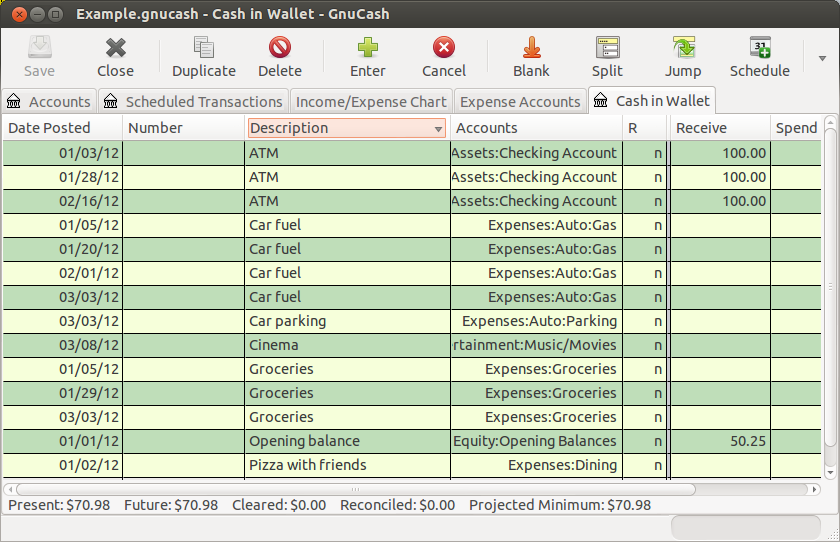
\includegraphics[width=\textwidth]{gnucash.png}
	\vspace{-0.8cm}
    \caption{Example GNU Cash UI \cite{GNUCashUI}}
    \label{fig:gnucash_ui}
\end{figure}

\subsection{Mobile Banking Applications}
\label{sec:mobile-banking-applications}
These applications are the default applications that come with each bank. Almost always, if the bank offers a website for online banking, they also offer a mobile application that perform the same functions. These include the major banks such as HSBC, NatWest, Lloyds etc., but also includes the online-only banks such as Monzo and Revolut. Sometimes, these applications do not use open banking as instead just display information about the accounts with that specific company, so do not need to use the services of other banks. There are some that do connect with other banks, but they often don't incorporate the information into the analytics, and instead just display the balances.

Taking Revolut \cite{RevolutWebsite} as a case study, we can find its strengths to incorporate, as well as its weaknesses to avoid in the web application. Firstly to even use the Revolut's app functionality, a user must open a bank account with the service and prove their identity. Although this does provide the user with confidence that their information is secure and personalised, it also means it is more difficult to use, slower to gain access to the information and overall just has a catch. It also means that the primary purpose of the app is not to provide a user with an overview of their finances, but instead to provide a banking service, so will not be aimed at improving financial capability. There are some features of Revolut which are worth acknowledging, such as the UI and ability to track expenditure. In having a slick and intuitive user interface, it enables users to understand all aspects of their finances and helps build confidence. The expenditure tracking is particularly useful, it allows users to customise a budget for a set time period and shows what and when they have spent money in during this period; overall aiming to help them stay within the budget. Revolut is a service that does utilise open banking as allows to you connect the app to other bank accounts, however it doesn't incorporate these into the budgets and only really includes them in the net worth section. This is a good example of a service that does use open banking, but doesn't utilise it to its full potential.

\subsection{Paid Applications}
\label{sec:paid-applications}
The final category of applications is really just the 'other' section, however the majority of these do incur costs to use. These applications are often more powerful than the free alternatives, yet are often filled with advertisements and are not as user friendly. A good example of this is Quicken which won the awards for the best budgeting app in 2020 and 2021 \cite{Quicken}, but costs up to \textsterling 10/month. It utilises open banking effectively to work with many different bank accounts, yet it does not enable quick-toggling of bank accounts to incorporate/ignore during the analysis and overview. This is a feature which would be particularly useful in giving analysis and a better overview as a user would be able to segment e.g. all the savings accounts. Despite having some effective budgeting features, it lacks the ability to perform budgeting prediction from patterns in expenditure. This feature also would be useful in improving financial capability because it will help the user plan for future expenses and identify areas where they can save money. Overall, these paid applications have some aspects which would be useful in the web application, but they also are missing some basic ones which would be more focused on improving financial literacy.

\section{Open Banking}
\label{sec:open-banking}
Open banking is defined as "APIs [that] enables third-party developers to build applications and services around the financial institution", in this paper \cite{OpenBankingDefinition}. The open banking movement, is therefore the recent pressure on banks to open up their data to third-party developers. They do this by creating a set of endpoints which developers can query, and will respond with accurate and live data. For example, a user would first login to their online bank via a popup, this would then return an authentication token which the website can use to query e.g. to get their recent transactions; the information is then returned in a secure response. Each bank has their own set of endpoints such that the authentication process and available information differs across them all. This is where a lot of problems arise as reading the documentation is not straightforward and time consuming, however it is necessary to enable the web application to support all the major banks. This lack of standardisation is where Plaid \cite{Plaid} come in.

\subsection{Plaid}
\label{sec:plaid}
Plaid is a platform that, effectively, wraps all the endpoints provided by each individual bank and provides a single standardised set of REST API endpoints as URLs. This means that the web application only needs to query Plaid, and in turn will be able to support all the banks that Plaid provide access to - over twelve-thousand institutions \cite{PlaidInstitutions}.

To use Plaid's endpoints, a strict authentication flow must be followed as it is handling very private data. Plaid has three different types of tokens as part of this flow. The first is the link token; Link is the name for the widget that is used to authenticate the user with their bank but to do so requires a link token. They can simply be requested from Plaid's API and are valid for 4 hours, but are not tied to any user and are not treated as passwords. Secondly, there are public tokens; these are what the link widget returns to the web application after the user has authenticated with their bank and so are unique to that user. They also are not treated as passwords as are valid for only 30 minutes and cannot be used to access a user's private information directly. They must be exchanged for an access token, which is the third type of token. This exchange is done via a Plaid endpoint but must be done via the web application's server, rather than client because the response access token must be treated like a password and be kept extremely securely. If it was done on the client, it risks being exposed and anyone with this token can access that user's information. Embedded within the access tokens can be a set of bank accounts, and a user may have several access tokens tied to them.

The flow is therefore: the client requests a link token on behalf of the user, the response link token is then passed to the link widget where the user signs in with their bank; the link widget returns a public token to the client which is passed to the application's backend; the backend exchanges the public token for an access token and then stores this in the database in such a way that only that user can access it. Whenever the client wants to gain access to that user's transactions, it queries the server acting as a proxy. The server identifies which user is asking for the information and attaches their access token to a new request to Plaid. The Plaid response is then forwarded back to the client and the client can display the information to the user. This flow is shown in Figure \ref{fig:plaid_auth_flow}.

\begin{figure}[H]
	\centering
    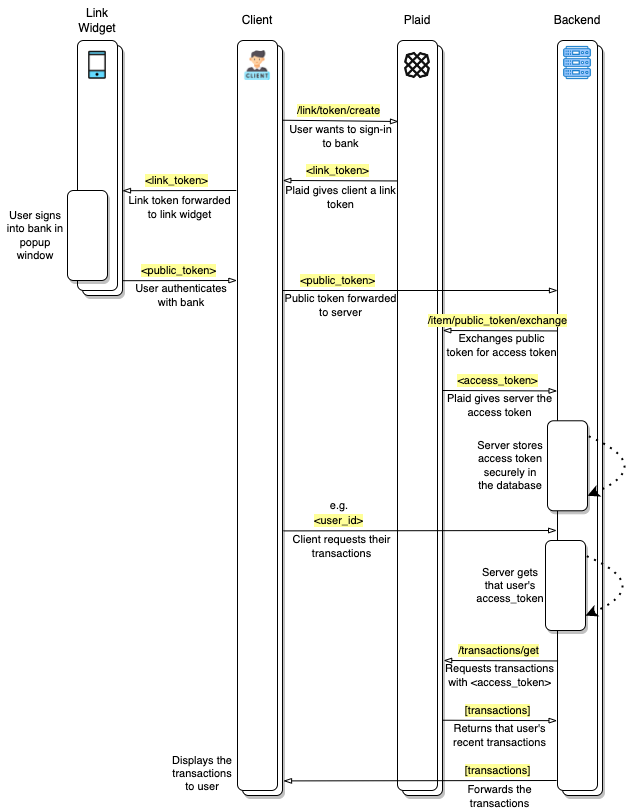
\includegraphics[width=\textwidth]{Plaid_auth_flow_sequence_diagram.png}
	\vspace{-0.8cm}
    \caption{Plaid Authentication Flow}
    \label{fig:plaid_auth_flow}
\end{figure}

Further aspects of Plaid relevant to this project include the different modes of operation. When the web application makes queries to Plaid's endpoints, one of three modes can be specified and each produce different results. The first is sandbox mode, this is the default that everyone has access to. All the endpoints and request formats remain the same, but the responses are fake data generated by Plaid themselves. This is useful for testing the web application without having to connect to a bank so do not have to worry about leaking any private information, as well as getting fast and reliable responses. The second is development mode where the responses are real data. The full authentication flow must be followed and a user will login to their bank. To gain access to this mode, it must be requested by Plaid and they review the application to check that it is secure and will not leak any information. Once given access, there is a limit of one-hundred user accounts connected to actual banks, so this had to be managed carefully. The final mode is production mode, this is the same as development mode but with no limits. To gain access to this, further vetting is required and the queries start to cost. For this project, only sandbox mode was initially used, then following the completion of the prototype, development mode was requested and given for further testing and demonstrations.

\section{Further Motivation}
As previously mentioned, the main motivation for this project came from the recent open banking movement, so using modern technology to help push the field. In addition to this, the limited current services available was also a factor as it was identified that there was a need for an application like this. Finally, the timing for this project is very appropriate as the UK government announced that there is a financial crisis currently going on, which they named the 'Cost of Living Crisis' \cite{CostOfLivingCrisisGov}. Furthermore, in the Money and Pensions Service's recent report, they advised that people get a budget planner to help cope with the current times. This then helped concrete an objective for the web application to include budgeting features, as would also help improve financial capability.